\section{Periglacální zóna}
Periglaciální zóna nebo také \enquote{příledovcová} zóna je prostředí, kde působí \emph{kryogenní} geomorfologické procesy. Nejedná se o území trvale pokryté ledem (ledovci), ale o území, které je po velkou část roku ovlivněno teplotami pod bodem mrazu. Periglaciální zóna je charakteristická přítomností \emph{permafrostu}. Přibližně čtvrtina zemské souše spadá do periglaciální zóny. 
%POdle charakteru klimatu můžeme rozlišit Rozlišujeme tři typy periglaciálního prostředí.
%\begin{itemize}
%	\item Oceánické (islandský typ)
%	\item Kontinentální (sibiřský typ)
%	\item Horské (alpinský typ)
%\end{itemize}

Rozsah současné periglaciální zóny je znatelně menší oproti pleistocénu, kdy existovaly rozsáhlé kontinentální ledovce. Na některých územích je permafrost reliktem -- pozůstatkem dob ledových. Neodpovídá tedy současným klimatickým podmínkám. 

\section{Permafrost}
\emph{Permafrost} je dlouhodobě zmrzlá část litosféry a pedosféry (tzv. kryolitozóna). Permafrost tak může být tvořen jak zeminami, tak i skalními horninami. Normativně je permafrost definován jako část litosféry a pedosféry jejíž teplota je minimálně dva roky pod \SI{0}{\degreeCelsius}. 

Permafrost vzniká v oblastech se zápornou tepelnou bilancí. Více tepla je z území vyzářeno, než se tam dostane slunečním zářením a tepelným tokem z nitra Země. Přítomnost permafrostu je tak soustředěna do vysokých zeměpisných šířek a vysokých nadmořských výšek. V současné době se permafrost nachází asi na $24 \%$ souše severní polokoule (Obr. \ref{fig:permafrostdistr}). Zahrnuje to především území Kanady, Aljašky a Sibiře a Grónska. Na jižní polokouli je permafrost rozšířen zejména na území Antarktidy.

\begin{figure*}[h]
	\centering
	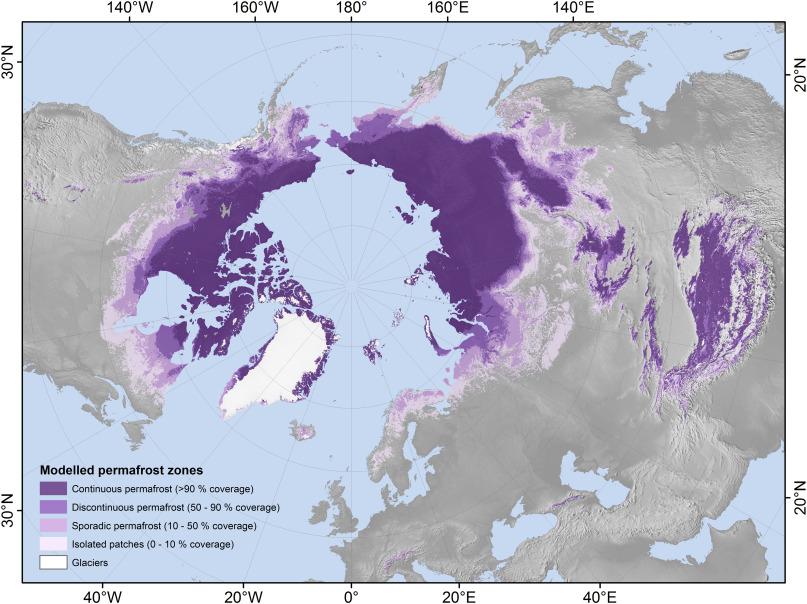
\includegraphics[width=1\linewidth]{obrazky/periglac/permafrost_distr}
	\caption{Distribuce permafrostu na severní polokouli (převzato z \textcite{obuNorthernHemispherePermafrost2019}).}
	\label{fig:permafrostdistr}
\end{figure*}

Permafrost dělíme podle jeho spojitosti do několika typů. \emph{Souvislý permafrost} představuje jednolitou masu zmrzlé horniny, kde k tání dochází pouze v aktivní vrstvě. \emph{Nespojitý permafrost} značí, že se v území nacházejí místa, která jsou trvale roztátá. \emph{Sporadický permafrost} označuje oblasti s občasnou přítomností permafrostu. 

Mocnost permafrostu se pohybuje zpravidla v desítkách metrů. Avšak v některých oblastech na Sibiři dosahuje mocnosti až \SI{1500}{\metre}. 

Permafrost může vzniknout po uložení sedimentu (klidně s odstupem tisíců či miliónů let). Takovýto permafrost nazýváme \emph{epigenetický}. Pokud ale dochází současně se sedimentací i k zamrzání, vzniká \emph{syngenetický} permafrost. Syngenetický permafrost vzniká například v aluviálních a deltových prostředích v severoamerické Arktidě (např. řeka Mackenzie) a v severní Sibiři (např. řeky Lena, Kolyma aj.). Rozdíl mezi epigenetickým a syngenetickým permafrostem je i ve směru, jakým roste s časem jeho mocnost. Epigenetický permafrost roste od povrchu směrem dolů (v závislosti na délce trvání příhodných podmínek). Syngenetický permafrost naopak roste vzhůru tak jak se na daném místě akumuluje další materiál.

Podle lokalit, kde se permafrost nachází ho můžeme rozdělit na pásemný (polární) permafrost, který se nachází ve vysokých zeměpisných šířkách, montánní nebo také permafrost náhorních plošin (typicky permafrost ve vysokých nadmořských výškách v Centrální Asii) a horský permafrost, který se nachází ve středních a nízkých zeměpisných šířkách ve vysokých nadmořských výškách (např. Alpy).

\begin{figure*}[h]
	\centering
	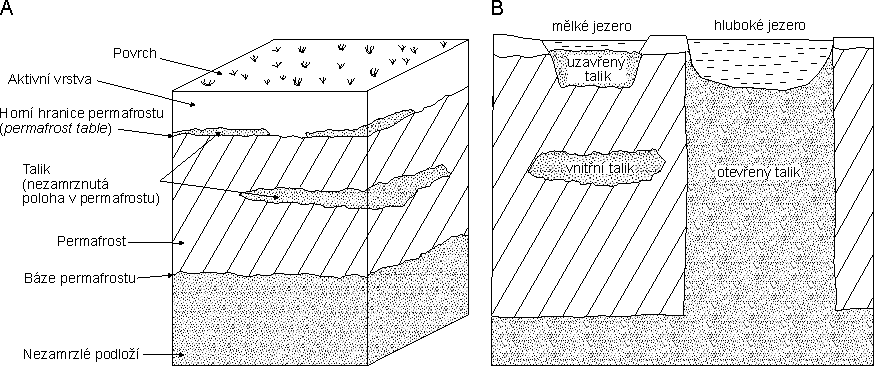
\includegraphics[width=1\linewidth]{obrazky/periglac/talik}
	\caption{A -- vymezení permafrostu, jeho horní hranice a báze (upraveno podle \textcite{jrPermafrostRelatedEngineering1969}), B -- rozdělení taliků na uzavřený (obklopen permafrostem zespod a ze stran), často pod mělkými jezery; otevřený talik (pod hlubokým jezerem či vodním tokem); vnitřní talik (upraveno podle \textcite{demekObecnaGeomorfologie1987})}
	\label{fig:talik}
\end{figure*}

\subsection{Aktivní vrstva}
\emph{Aktivní (činná) vrstva} je přípovrchová vrstva, která pravidelně (sezónně) taje. V jejím podloží je permafrost. Mocnost aktivní vrstvy se pohybuje v řádu prvních decimetrů (polární oblasti) až po více jak metrové mocnosti v subarktických oblastech. Mocnost aktivní vrstvy je ovlivněna celou řadou faktorů jako je například teplota vzduchu, vegetační kryt, mocnost sněhové pokrývky, obsahu vody, typ hornin, orientace a sklon svahu. I proto se mocnost aktivní vrstvy může rok od roku lišit. Jelikož zmrzlé podloží brání vsakování vody do větších hloubek, je aktivní vrstva zpravidla saturovaná vodou. V nezpevněných sedimentech tak má podobu rozbředlé zeminy. 

Tání aktivní vrstvy probíhá vždy od povrchu směrem do hloubky. K zamrzání aktivní vrstvy dochází ale ze dvou směrů. Jak od povrchu směrem do hloubky ale i opačným směrem, kdy aktivní vrstva zamrzá od permafrostu vzhůru. 

Mezi aktivní vrstvou a samotným permafrostem můžeme vymezit ještě přechodnou vrstvu, která taje jen během extrémně teplého léta. Tato přechodná vrstva je zpravidla bohatá na podzemní led.

\begin{figure*}[h]
	\centering
	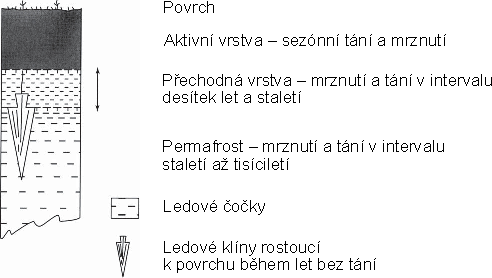
\includegraphics[width=0.7\linewidth]{obrazky/periglac/aktivni_vrstva}
	\caption{Model rozhraní aktivní vrstvy a permafrostu o třech vrstvách. Aktivní vrstva taje a zamrzá sezónně. Přechodná vrstva roztává a zamrzá v horizontu desetiletí až staletí. Permafrost je dlouhodobě zmrzlý a jeho tání a zamrzání je otázkou staletí až tisíciletí (upraveno podle \textcite{frenchPeriglacialEnvironment2017})}
	\label{fig:aktivnivrstva}
\end{figure*}


\subsection{Talik}
V permafrostu se vyskytují polohy, které nejsou zamrzlé. Označují se jako \emph{talik}. V sedimentech jsou často nasyceny vodou. Taliky můžeme rozdělid do tří druhů. \emph{Uzavřený talik} je na bocích a zdola obklopen permafrostem. Nad ním je aktivní vrstva. \emph{Otevřený talik} sahá od aktivní vrstvy až po bázi permafrostu. \emph{Vnitřní talik} je ze všech stran obklopen permafrostem. 

\subsection{Podzemní led}
Ve většině hornin a zemin je přítomná voda, která zamrzá a mění se v podzemní led. Pokud voda není přítomna a jedná se jen o zmrzlé horniny hovoříme o tzv. suchém permafrostu. Zamrzající voda významně ovlivňuje celou řady vlastností materiálu (fyzikálních, chemických, tepelných apod.). Sypký materiál je ledem zpevněn.

Podzemní led má celou řadu podob. Významný je zejména v nezpevněných sedimentech.  \emph{Texturní led} (pórový, cementační) je součástí horniny a spojuje tak jednotlivé částečky. Je tvořen drobnými ledovými krystaly (desetiny milimetru až první centimetry). Jedná se o vodu, která se nachází v sedimentu a mrzne \textit{in situ}. Druhým základním typem podzemního ledu je tzv. \emph{masivní led}. Do této skupiny řadíme několik podtypů. \emph{Segregační led} vzniká v sedimentech, které jsou ve velké míře saturované vodou. Vytváří ledové čočky o rozměrech od několika milimetrů až po velká tělesa někdy až i desítky metrů mocná. \emph{Intruzivní led} vzniká proniknutím vody do horniny pod tlakem. \emph{Žilný led} se vytváří díky pronikání povrchové vody do trhlin, které v permafrostu vznikají mrazovou kontrakcí. Tímto způsobem vznikají ledové klíny. Kromě výáše uvedených základních typů podzemního ledu existuje i celá řada dalších. Led může vyplňovat dutiny v horninách (např. jeskynní led). \emph{Pohřbený led} vznikl na povrchu a následně byl překryt sedimenty.

\section{Kryogenní procesy}
Voda při přeměně v led zvětšuje svůj objem o přibližně $9 \%$, což vyvolává znatelné napětí v horninách, pokud voda nemá kam expandovat. Například když voda nateče do puklin, které zamrzají zvenku. Jinou variantou je vznik segregačního ledu, který způsobuje vertikální a horizontální pohyby klastů ve zvětralinách. Jedná se o nesouvislé čočky ledu, které vznikají při mrznutí činné vrstvy. 

\emph{Kryoturbace} je proces promíchávání nehomogenních zvětralin v důsledku promrzání vody v sedimentech. 
Opakované zamrzání a rozmrzání, růst ledu vede k \emph{mrazovému tříštění} (kongelifrakci) hornin. Klasickým produktem mrazového tříštění jsou rozsáhlá \emph{kamenná moře}. 

\begin{figure}[h]
	\centering
	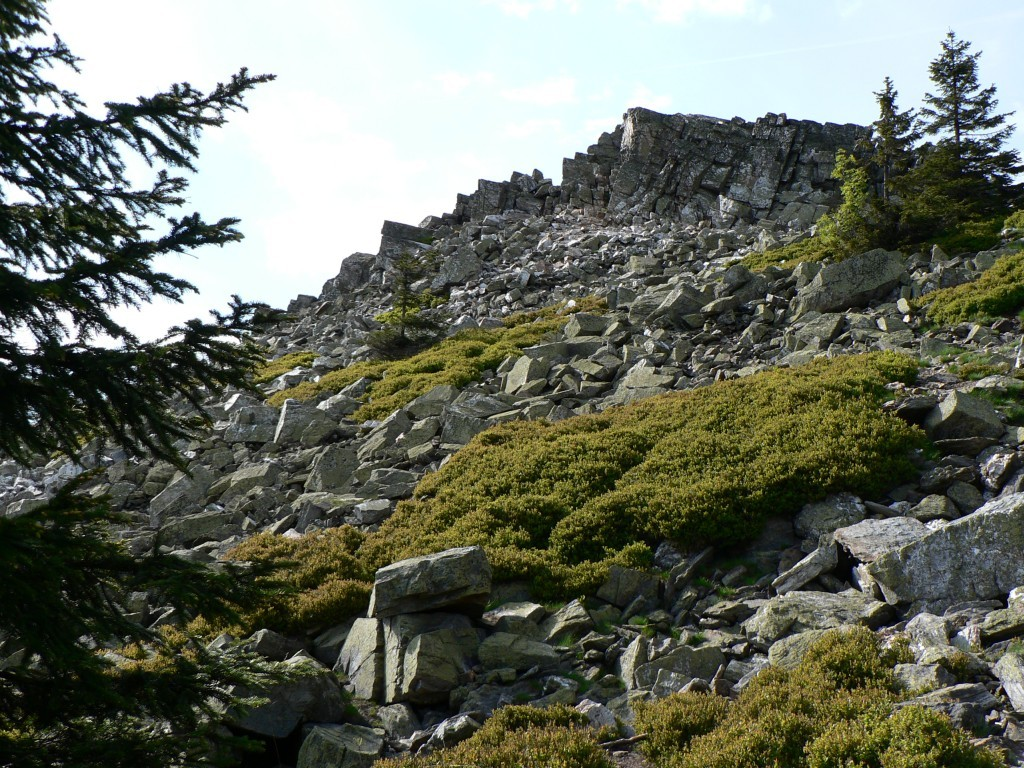
\includegraphics[width=1\linewidth]{obrazky/periglac/kamenne_more}
	\caption{Kamenné moře na Ztracených kamenech, Jeseníky (autor: Martin Vavřík – Vlastní dílo, Volné dílo, via Wikimedia Commons)}
	\label{fig:kamennemore}
\end{figure}

Na svazích i o malém sklonu dochází k \emph{soliflukci} (\textit{solifluction}), což je pomalé ploužení zemin. Termín soliflukce zastřešuje celou několik procesů (Obr. \ref{fig:soliflukce}): ploužení způsobené jehličkovým ledem (Obr. \ref{fig:jehlickovyled}), mrazové ploužení, geliflukci. Typickým výsledným projevem soliflukce jsou tzv. \emph{soliflukční laloky} (\textit{solifluction lobes}, Obr. \ref{fig:soliflukcnilaloky}).

\begin{figure}[h]
	\centering
	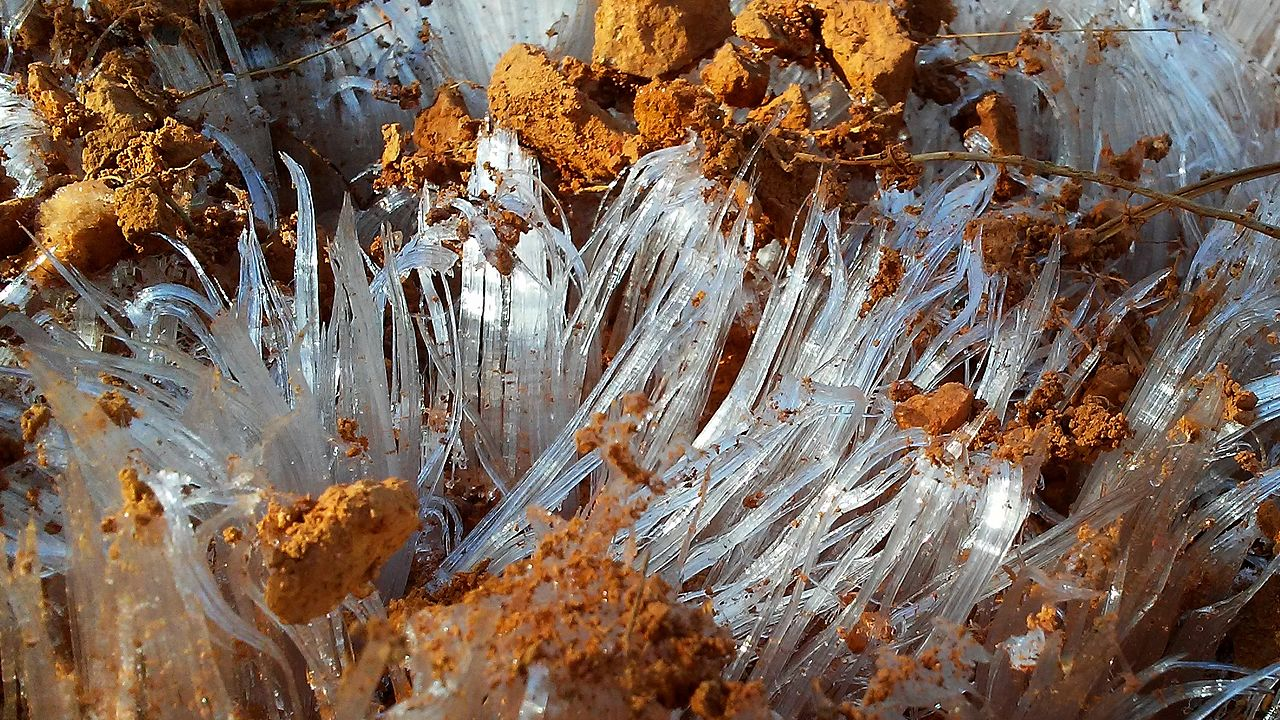
\includegraphics[width=1\linewidth]{obrazky/periglac/jehlickovy_led}
	\caption{Jehličkový led (\textit{needle ice}). (Foto: Wasrts, CC BY-SA 4.0, Wikimedia Commons))}
	\label{fig:jehlickovyled}
\end{figure}

\begin{figure}[h]
	\centering
	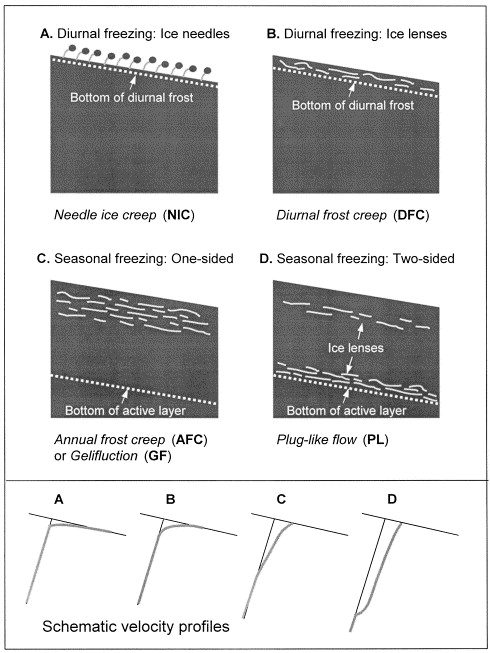
\includegraphics[width=1\linewidth]{obrazky/periglac/soliflukce}
	\caption{Procesy uplatňující se při soliflukci. \parencite{matsuokaSolifluctionRatesProcesses2001}}
	\label{fig:soliflukce}
\end{figure}


\begin{figure}[h]
	\centering
	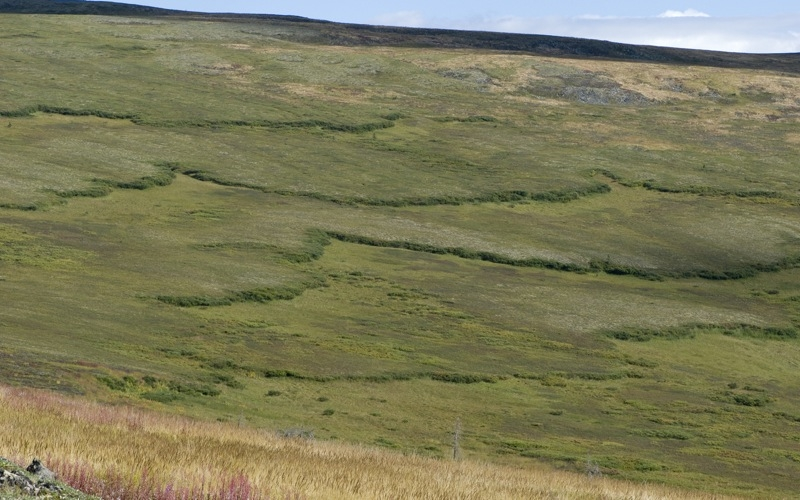
\includegraphics[width=1\linewidth]{obrazky/periglac/soliflukcni_laloky}
	\caption{Soliflukční laloky (Foto: D. Sikes CC BY-SA 2.0)}
	\label{fig:soliflukcnilaloky}
\end{figure}

Na březích vodních toků, jezer a oceánů dochází k intenzivní erozi vlivem mechanického (\emph{termoabraze}) a termického (\emph{termoeroze}) působení vody. Výsledkem je rychlé ustupování břehů. 

%\subsection{Agradace a degradace permafrostu}
%\emph{Agradace permafrostu} znamená zvětšování jeho mocnosti. 

\section{Periglaciální tvary reliéfu}
\subsection{Tvary v zeminách}
\emph{Strukturní} (kryogenní) půdy jsou specifické tvary reliéfu, které vznikají v důsledku mrazového třídění. Mohou mít podobu více či méně vytříděných kruhů (Obr. \ref{fig:strukturni_kruh}), polygonů (Obr. \ref{fig:strukturni_polygon}), pruhů či stupňů. Jejich vznik a podoba je závislá na sklonu svahu, materiálu a dalších. Fosilní strukturní půdy se nacházejí například v Krkonoších a Jeseníkách.

\begin{figure}
	\centering
	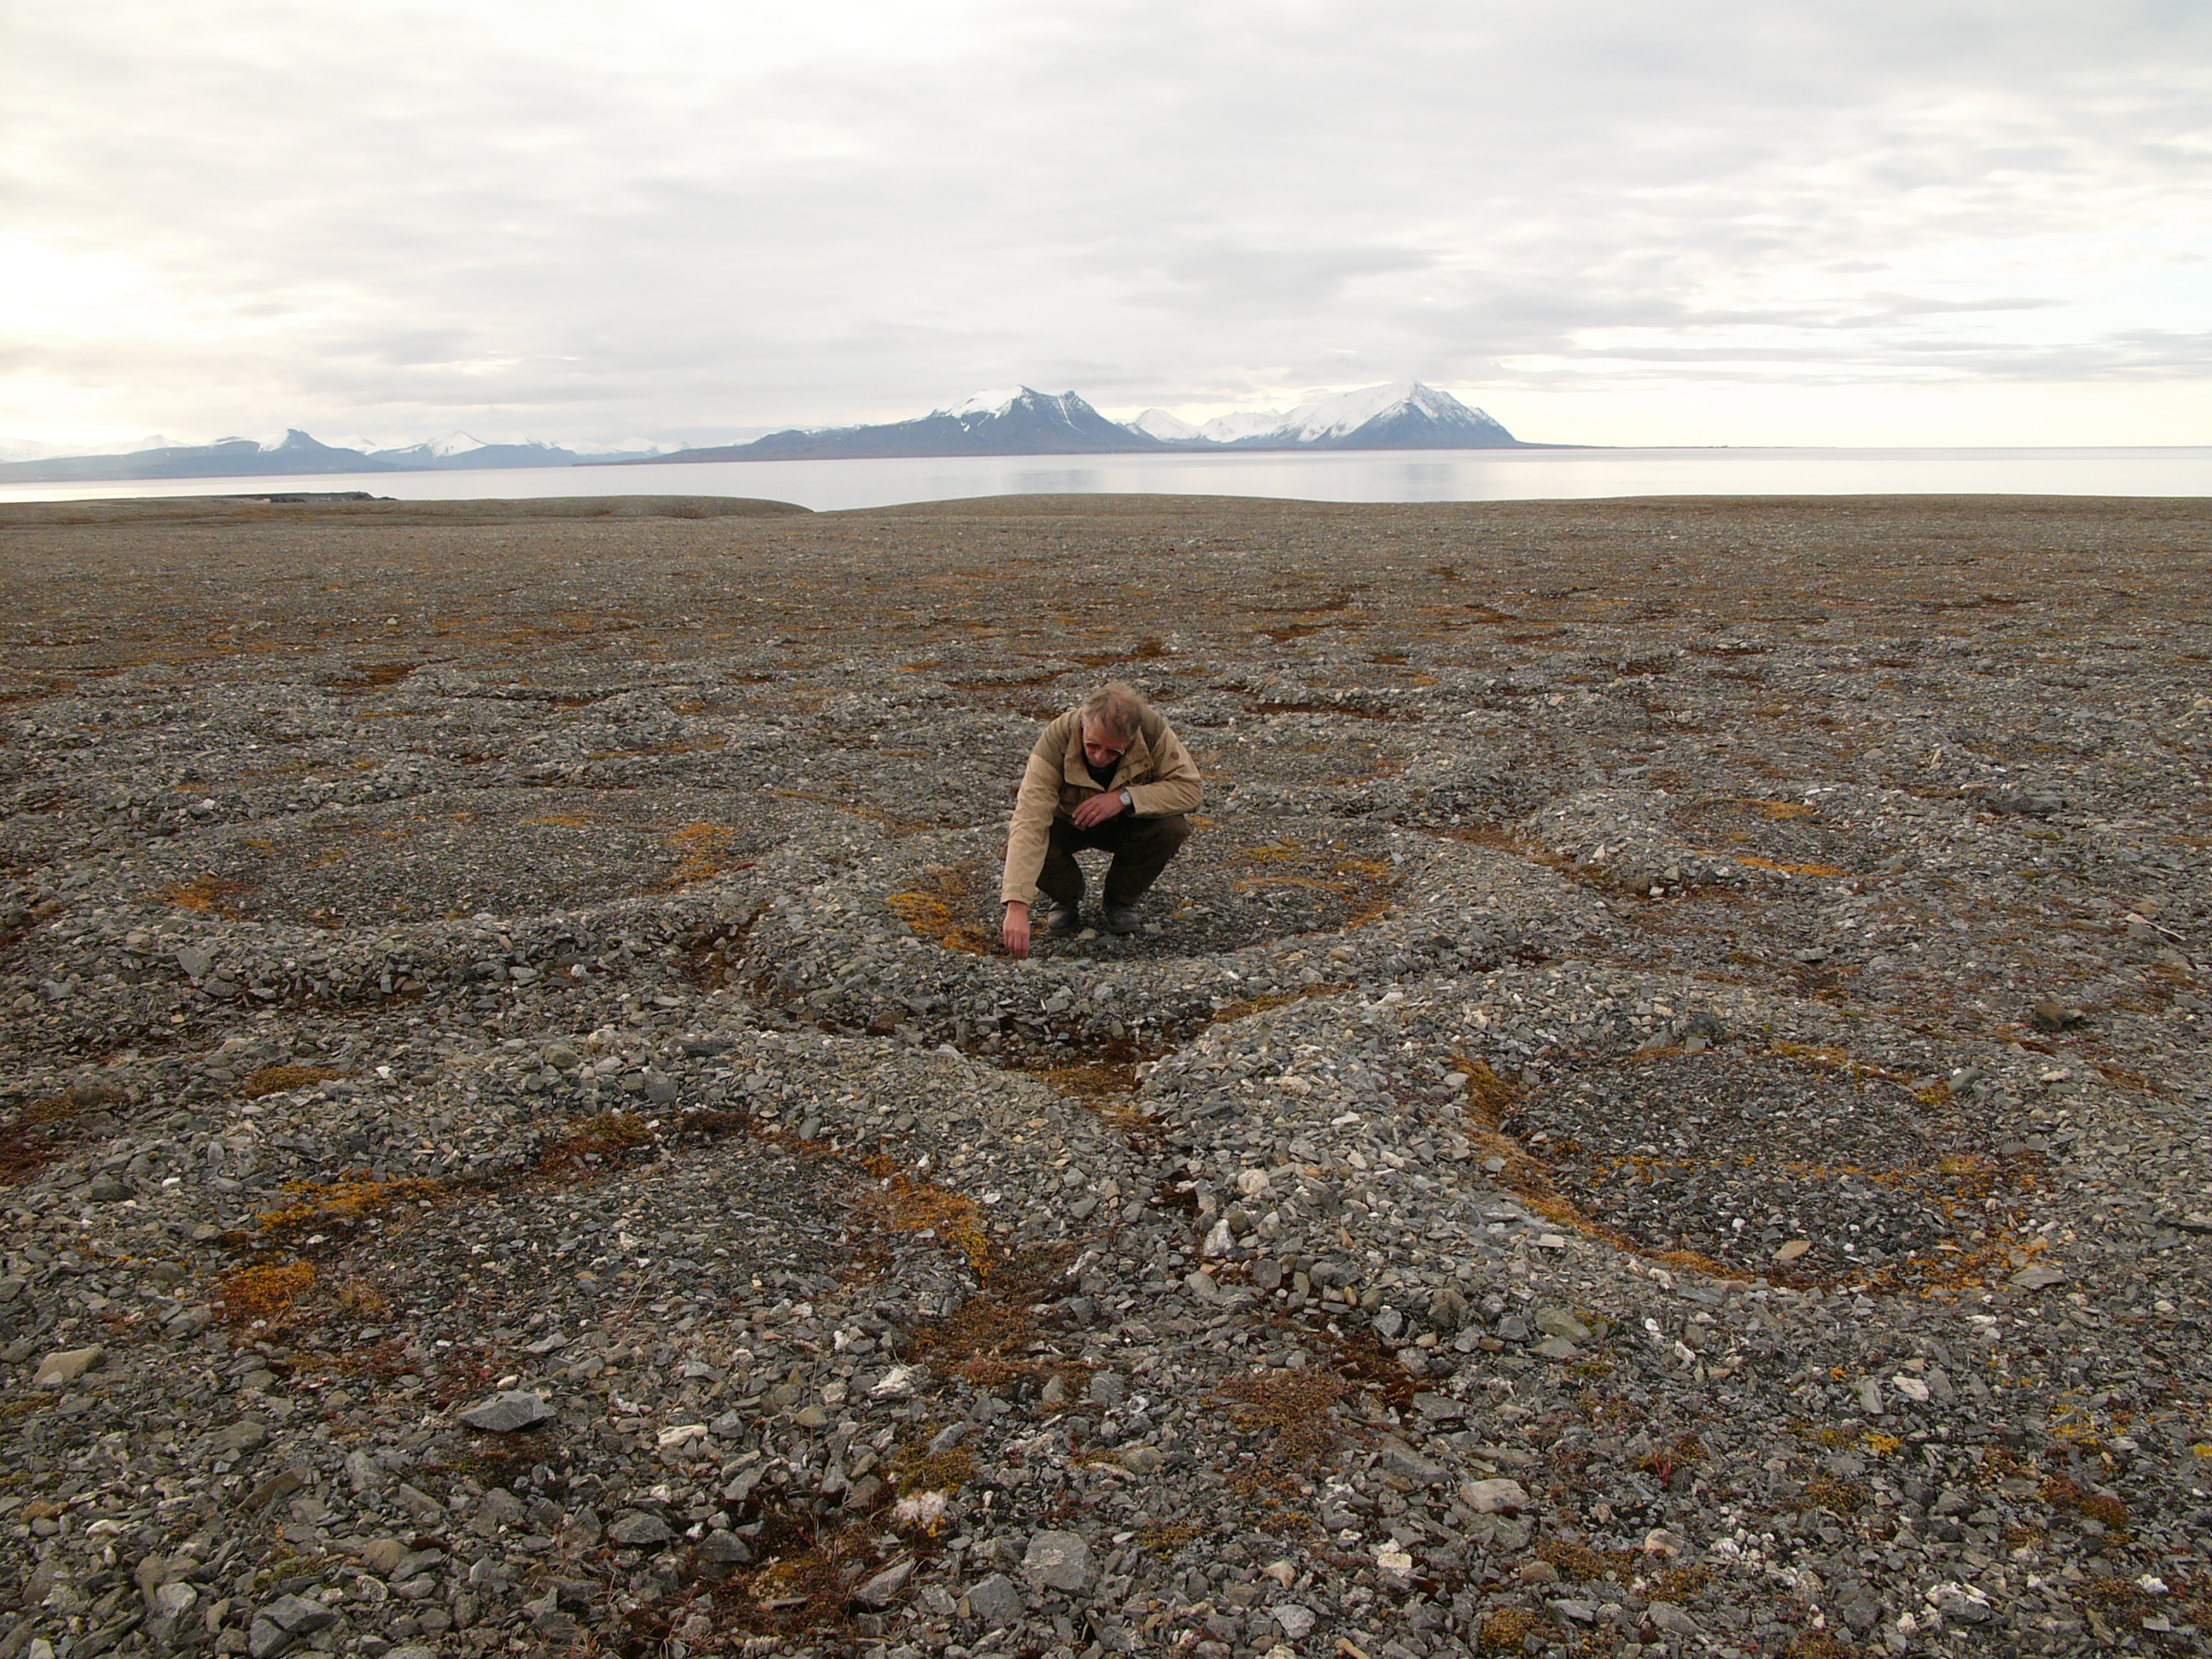
\includegraphics[width=1\linewidth]{obrazky/periglac/polygony}
	\caption{Kamenné kruhy, Špicberky (Hannes Grobe, CC-BY-SA-2.5)}
	\label{fig:strukturni_kruh}
\end{figure}

\begin{figure}
	\centering
	\includegraphics[width=1\linewidth]{obrazky/periglac/polygon}
	\caption{Kamenné polygony, Špicberky (foto: Autor)}
	\label{fig:strukturni_polygon}
\end{figure}

\emph{Pingo} (Obr. \ref{fig:pingo}) je drobná vyvýšenina na povrchu permafrostu. Výška pinga je řádově metry až desítky metrů.  Vznikají promrznutím vody v taliku, čímž se zvětší objem a dojde tak k vyklenutí povrchu. Pingo má ledové jádro. Rozlišujeme dva typy: i) pingo vzniklé z otevřeného taliku (nad jezery) a ii) pingo z uzavřeného taliku (injektáž vody). Rozměrově drobnější analogií jsou sezónní pahorky z rašeliny nazývané \emph{palsa}.

\begin{figure}[t]
	\centering
	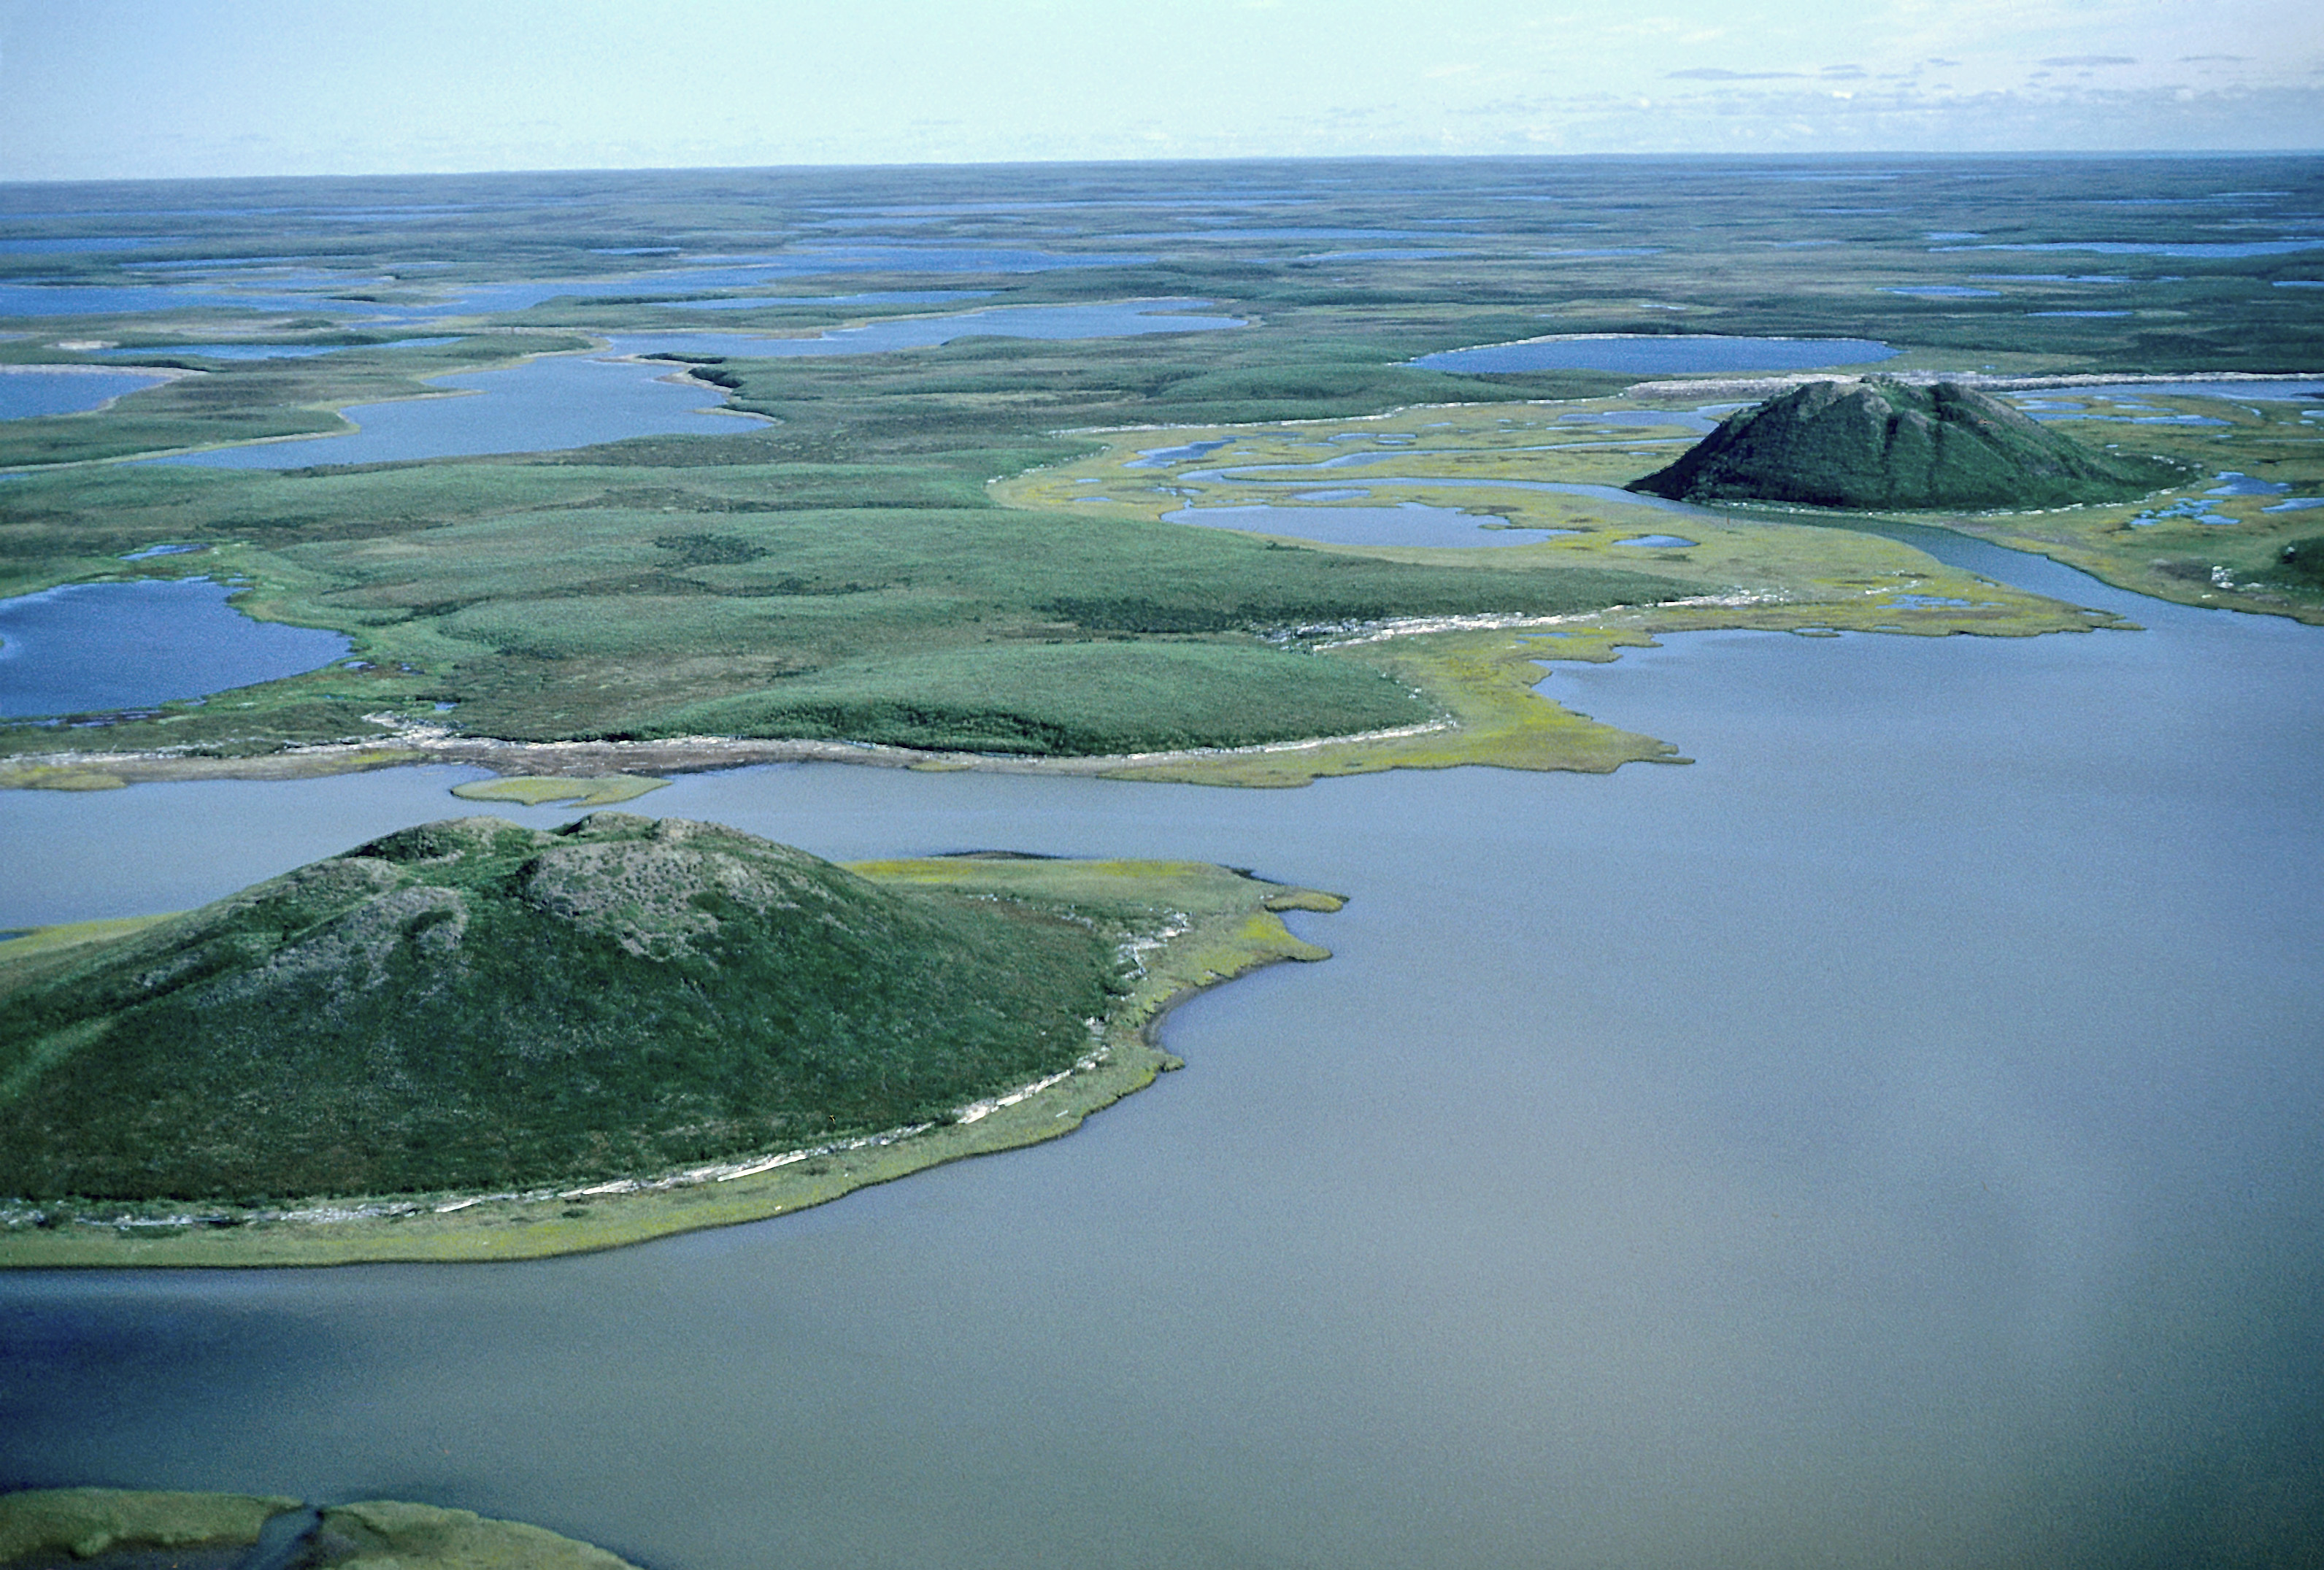
\includegraphics[width=1\linewidth]{obrazky/periglac/pingo_mackenzie}
	\caption{Pinga v deltě řeky Mackenzie (Autor: Lorenz King, CC)}
	\label{fig:pingo}
\end{figure}

\emph{Thufury} jsou dalším typem elevace. Jedná se o drobné kopečky (do cca \SI{2}{\metre}) s minerálním jádrem, které bývá často promrzlé. Nejčastěji se vyskytují v horských polohách jako jsou sedla nebo vrcholové plošiny. Pro vznik thufurů je nutná půdní vlhkost. 

Degradací permafrostu vznikají různé \emph{termokrasové tvary}. Jedná se především o různé sníženiny a zvlněný terén mezi nimi. Jejich rozsah je dán velikostí degradace permafrostu a množstvím podzemního ledu v zeminách. Termokras se významně vyvíjí v oblastech s množstvím ledových klínů. Postupným vývojem může být termokras ovlivňován i proudící vodou. K degradaci permafrostu může docházet shora nebo z boku. Degradace shora probíhá v plochém reliéfu. Započíná táním mrazových klínů a následným sesedáním povrchu. Vznikají deprese, které mohou být vyplněny jezerem -- \emph{alasy} (Obr. \ref{fig:alas}). Voda urychluje tání permafrostu, jelikož dokáže akumulovat velké množství tepla. Pod jezerem tak vzniká talik. Alasy mají běžně rozměry od několika metrů až do několika kilometrů. Po vyprázdnění jezera nebo jeho zanesená dochází k opětovnému promrzání taliku, což může vést ke vzniku pinga a polygonů ledových klínů. V členitém terénu dochází k degradaci z boku. Táním ledových klínů vznikají erozní rýhy. Ve svahu mohou vznikat i rozsáhlejší deprese nazývané \emph{termokary}. V nich bývá často exponovaný podzemní led.  Spojením alasů vznikají protáhlé sníženiny -- \emph{termokrasová údolí}. 

\begin{figure}[t]
	\centering
	\includegraphics[width=1\linewidth]{obrazky/periglac/alas}
	\caption{Termokrasová jezera na Sibiři. Snímek pořízený družicí Landsat (NASA, Public domain).}
	\label{fig:alas}
\end{figure}

Přítomnost permafrostu dala vzniknout v současnosti \emph{suchým údolím}. Jelikož permafrost fungoval jako izolant, tedy bránil vodě aby prosakovala do hlubších poloh, což způsobovalo povrchový odtok. \emph{Nesouměrná (asymetrická) údolí} vznikla rozdílnou intenzitou kryogenních pochodů na svazích s odlišnou expozicí. Na jižních a západních svazích se nedrží dlouho sněhová pokrývka, kryogenní pochody tedy intenzivně probíhají na jaře a po zbytek roku ustávají. Sníh na severních a východních svazích taje pomalu. Kryogenní pochody tak působí i přes léto. Materiál z těchto svahů odtlačuje vodní tok k protějším svahům, které eroduje a stávají se tak příkřejšími. Proto jižní a západní svahy těchto údolí jsou příkřejší než severní a východní. Údolím podobný, ale značně mělký tvar je \emph{úpad} neboli \emph{dellén}. Má ploché dno a mírné svahy. Jeho vznik bývá spojen s termokrasovými pochody nebo korazí. 

\emph{Skalní (kamenné) ledovce} (\textit{rock glaciers}) jsou rozsáhlé lalokovité akumulace klastického materiálu, který je stmelen podzemním ledem (Obr. \ref{fig:skalni_led}). Často se jedná o pohřbené zbytky ledovce. Podobně jako klasické ledovce se i skalní ledovce pomalu plasticky pohybují (tečou). Skalní ledovce nacházíme ve vysokohorských oblastech. Mohou být jak fosilní (již se nepohybují) nebo aktivní. 

\begin{figure}[t]
	\centering
	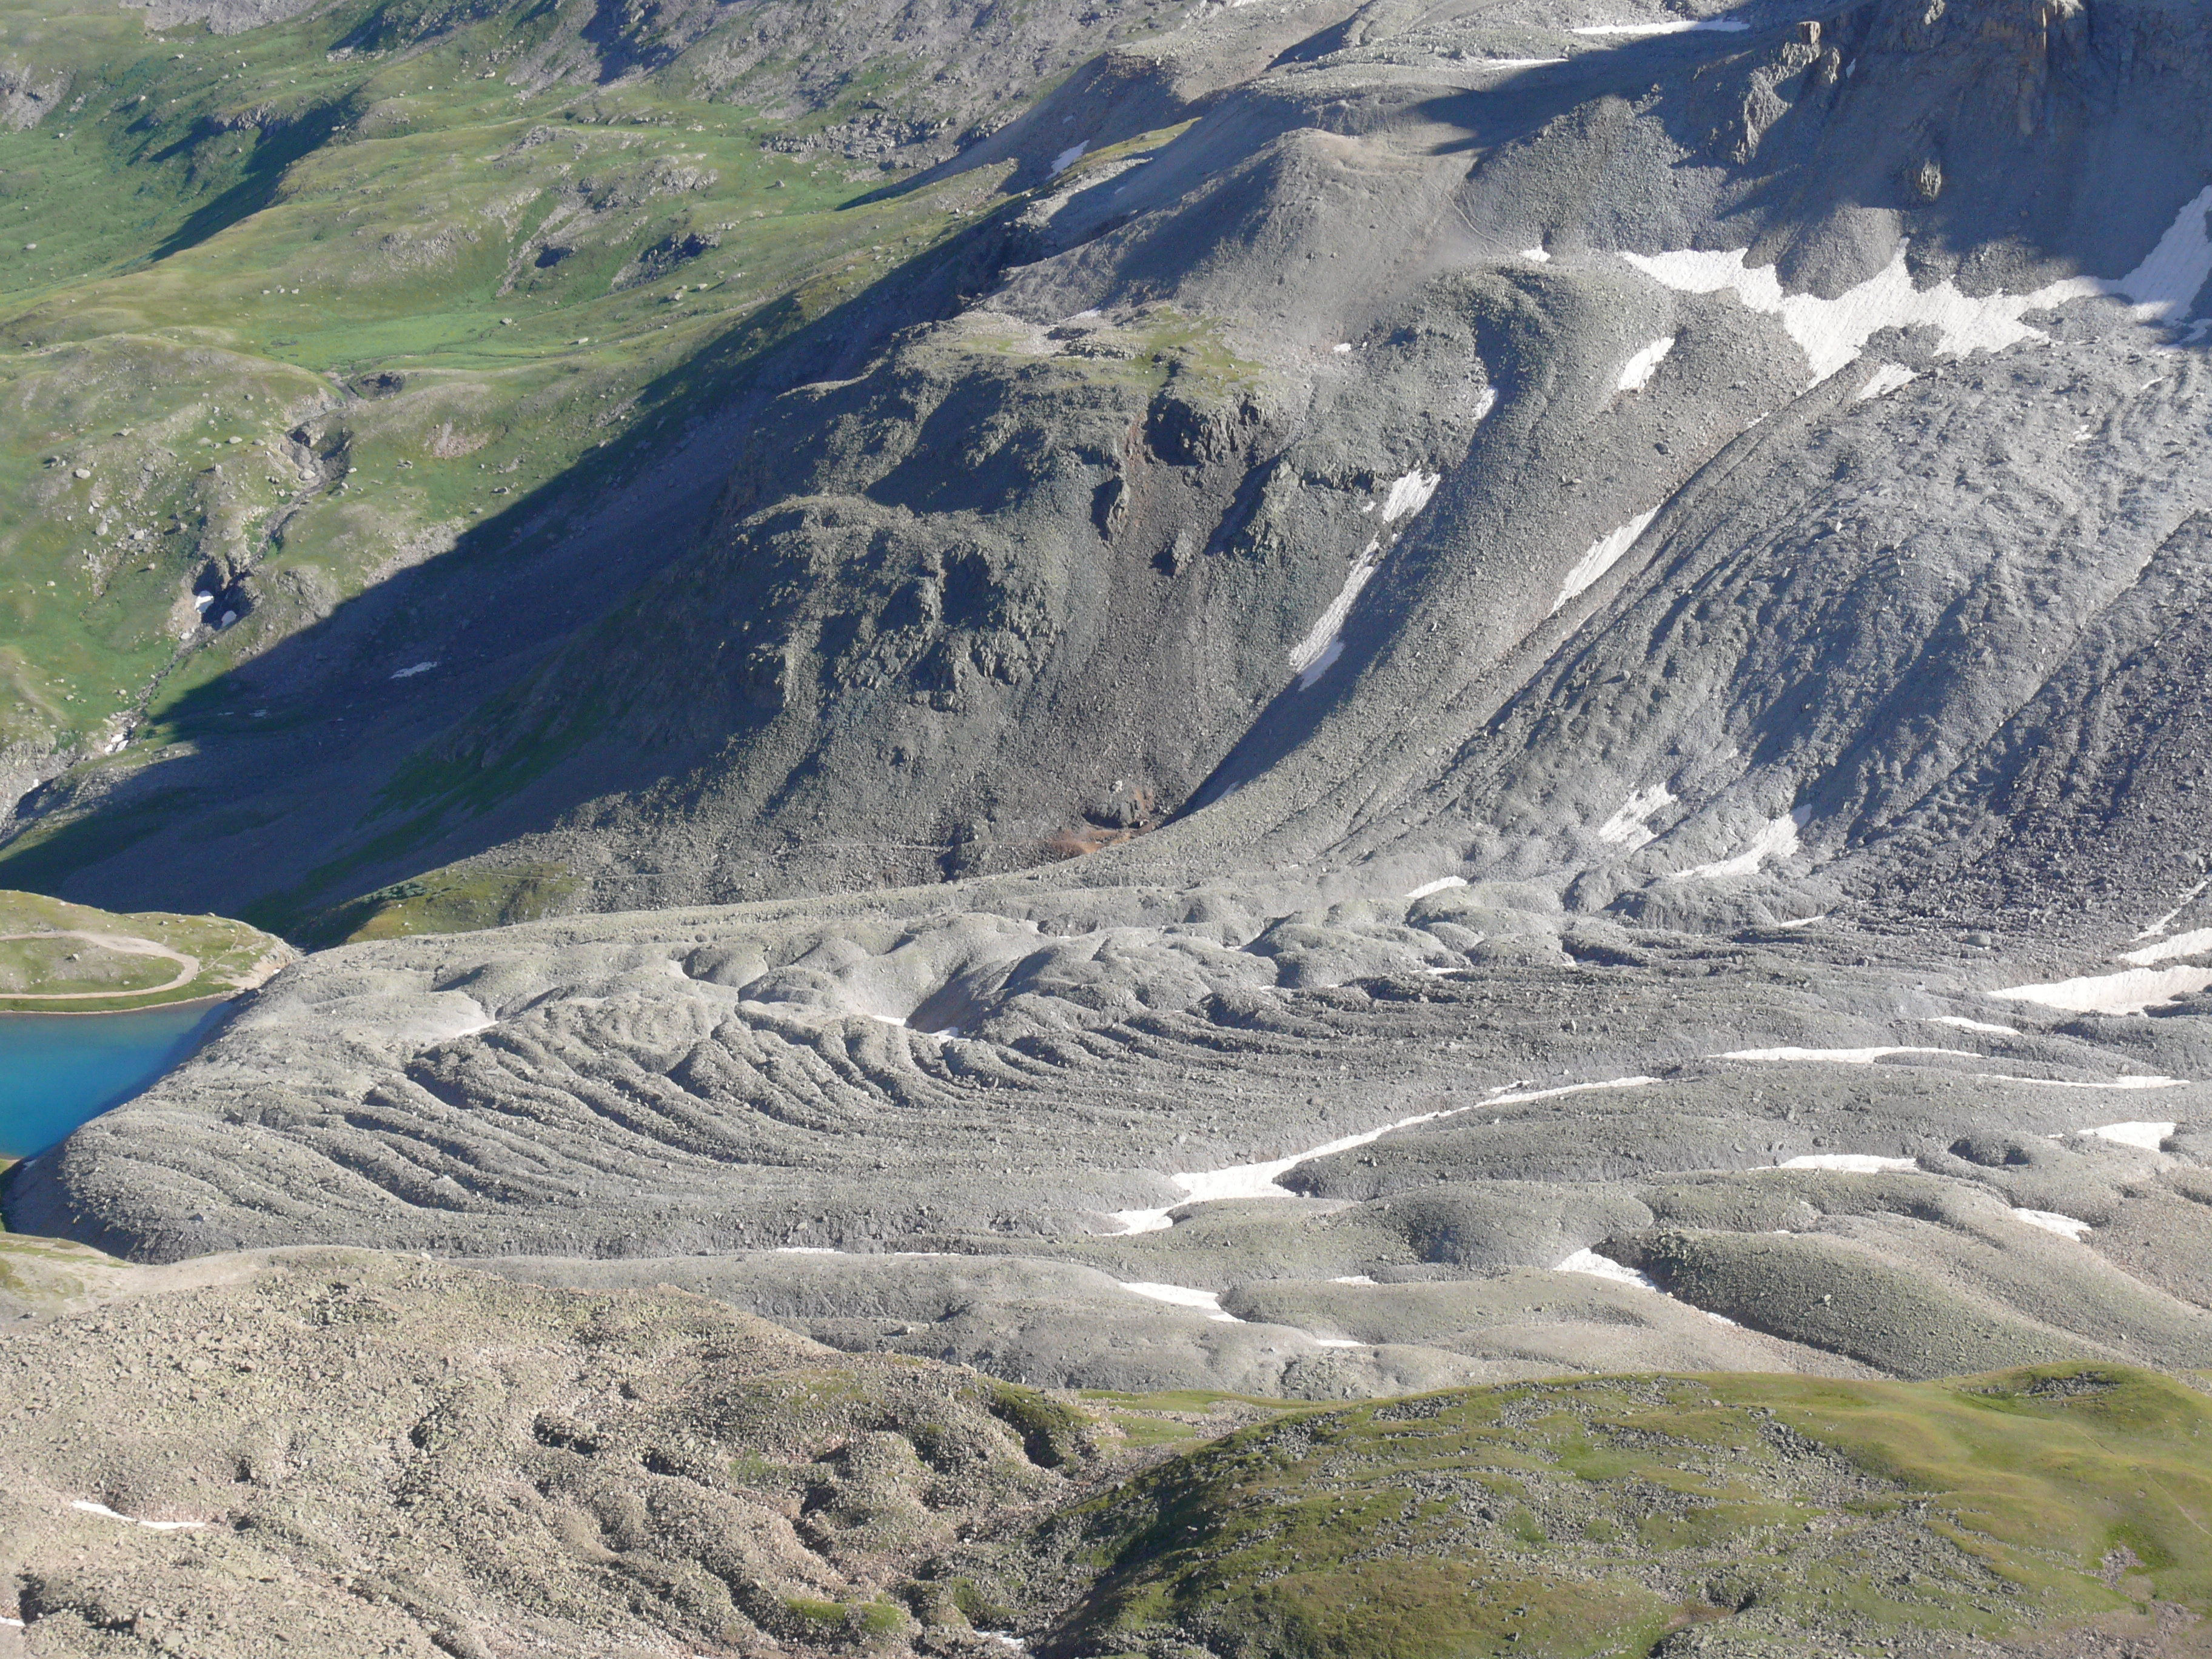
\includegraphics[width=1\linewidth]{obrazky/periglac/rock_glac}
	\caption{Skalní ledovec (Autor: Bob Webster, CC BY 2.0)}
	\label{fig:skalni_led}
\end{figure}

\subsection{Tvary ve skalních horninách}
Kryogenní pochody na svazích vedou ke vzniku \emph{kryoplanačních teras}. Jedná se o zpravidla mírně ukloněné plošiny, které jsou zaříznuté do skalního podloží. V horní části jsou ukončené stupněm -- mrazovým srubem. Šířka kryoplanačních teras se pohybuje od několika metrů až po desítky metrů. Jejich povrch je pokryt ostrohrannou sutí. Mohou se vyskytovat samostatně nebo ve skupinách. 

\emph{Mrazový srub} je příkrý ($>$\SI{80}{\degree}) až převislý. Jeho výška je v řádu metrů. Vývoj kryoplanačních teras a mrazových srubů je spojen s nivací. 

\emph{Nivace} je souhrnné označení pro geomorfologický účinek \emph{sněžníků} (sněhových akumulací) v \emph{nivačních depresích}. V těchto sníženinách dochází k intenzivnějšímu zvětrávání kvůli zvýšené vlhkosti a častému střídání regelačních cyklů (mrznutí/tání).  Spojením nivačních depresí vzniká iniciální kryoplanační terasa, která se pak dál rozšiřuje. Postupným sbližováním mrazových srubů na protilehlých svazích a jejich následným spojením na hřbetu vznikají \emph{skalní hradby} a izolované skály \emph{tory}. Ve finálním stádiu vývoje kryoplanačních teras dochází k jejich spojení v tzv. \emph{kryoplén}.

Akumulací materiálu na úpatí sněžníků vznikají \emph{nivační valy} (\textit{protalus rampart}).
\begin{figure}
	\centering
	\includegraphics[width=1\linewidth]{obrazky/periglac/protalus_rampart}
	\caption{Vznik protalus rampart -- akumulace na úpatí sněžníku}
	\label{fig:protalusrampart}
\end{figure}


\subsection{Skalní ledovce}
Skalní ledovce jsou tvary tvořené sutí a ledem. Často se jedná o terminální stádia horských ledovců.  


%\newpage
%\onecolumn
%\begin{boxotazky}{Kontrolní a klíčové otázky, na které bychom měli znát odpověď}
%	\begin{itemize}
%		\item 
%		\item 
%		
%	\end{itemize}
%\end{boxotazky}
%
%\begin{boxslovnik}{Další klíčové pojmy k zapamatování}
%	aaa & adfasd \\
%	
%\end{boxslovnik}
%\twocolumn